\section{Trust Management}
\label{sec:trust-management}
A Trust is being able to depend on something or someone completely knowing that
what you believe to be true is true. Trust has been interpreted as reputation,
trusting option, probability etc. \autocite{Liu2006} and it plays a vital role in an
organization.  In every organization, employee trust plays a pivotal role and
the trust issues can make or break the culture of organization. There is a lot
stress involved in working in an environment where the data is highly secured
and the trusts between the employees are minimal.  If there is no trust, then
the organization is not up to its standard. Hence a trust has to be developed
between the employees for the organization to be successful. 

\subsection{Data Transmission based on Trust}
In this model we develop the trust between the nodes and the transmission of the
data across various nodes is done by evaluation of a new value called “Trust
value”. A “Security Agent” is an agent who has an access to view the trust
values of the nodes at a particular node level. The security agent will monitor
the trust values of the nodes and communicate with the other security agent
within the network. Once the other security agent receives the trust value, he
approves based on certain criteria and gives permission to the node. Thus the
data transmission is done between nodes. The representation of transmission of
a single document from Node ‘A' to Node ‘B' is shown in the below Figure 1.


Initially the Node “A” gives the document classification type along with its
trust value to the Security Agent at that level which is level –I in this case.
The classification of the document is evaluated from the classification process
described above and it is divided into various categories. The Security agent at
level –I communicate with the Security agent at level –II and enquire for the
trust value of Node ‘B'. The Security agent at level –II monitors and gets the
trust value of Node ‘B'. The Security agent at level –I verify on certain
assumptions and gives approval to Node ‘A' and document is sent to Node ‘B'.
Now, in an organization there are number of employees and are working at various
levels like Chief Manager, Manager, Senior Associate, Associate, Junior etc.
Based on this hierarchy we have divided the group of nodes to be at each level
and these groups of nodes are maintained by one Security Agent. Now each
security agent will have number of nodes connected and all the security agents
together are linked to a single “Trust Server”. Now the communication between
the security agents is done through Trust server which will have the access to
get the trust values at each level. Each node will be involved in transmission
of data to its neighboring nodes as well as the nodes at various levels. The
Figure 2. explains the steps of transmission of data from Node ‘A' at level –I
to Node ‘B' at level –II and also to Node ‘C' at level –III. The Node ‘A' at
level –I decides to send data to Node ‘B' at level –II and also to Node ‘C' at
level –III. Node ‘A' gives the classification type of the data to the security
agent at level –I along with its trust value. The security agent at level –I in
turn communicate with the Trust server and requests for the trust values of Node
‘B' and Node ‘C'. Node ‘B' in the below scenario sends five documents to B1, B2,
B3, B4 and B5 respectively. Each time B sends the document and the trust value
is calculated. The trust value of the respective node should be updated every
time because anytime a request can come from any node of another level for data
transmission. Similarly Node ‘C' sends five documents to its neighbors C1, C2,
C3, C4 and C5 in this scenario and updates its trust value each time. The
security agent at level – II and level –II monitor the respective Node ‘B' and
Node ‘C's interaction with its neighboring nodes and gets the updated trust
values. These trust values are sent to the Trust server and communicated with
the security level – I. Based on the trust values, the Node ‘A' decides whether
to send the particular classified data to the Nodes ‘B' and ‘C'. Once the
transmission of the data is done, the Node ‘A's trust value is updated.

\begin{figure}[h!]
    \label{fig:TrustTransmission}
    \begin{center}
        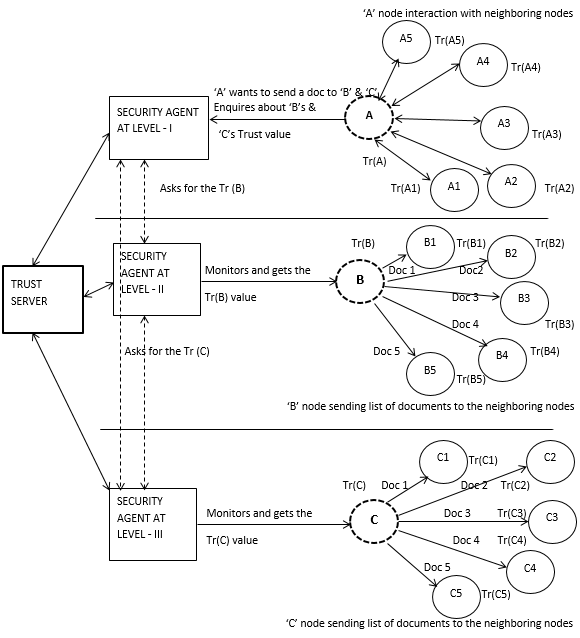
\includegraphics[width=0.90\textwidth]{Figures/Trust_Propagation_Diagram.PNG}
        \caption{Trust Value Propagation}
    \end{center}
\end{figure}


Impact of Trust values
We have criteria that when the Node interacts and data transmission is done, its trust value is reduced. The reduction in the trust value is based on the below points:
	When a Node sends a high secret data to another node which is not trusted (based on the trust value), then the nodes trust value is reduced by a high value.
	When a Node sends a high secret data to another trusted node, then the nodes trust value is reduced by a minimum value.
Trust Computation Factors
To compute the trust value, we took various factors in consideration. Few of them are listed below
	The Classification of the data which has to be sent to other node.
	The Similarity of the data meaning how much percentage of the data has been copied or used in another document.
	The old trust value, every time the node interacts with its neighbors, its old trust value is updated.
	The total number of documents shared by a particular node at a particular instance.

    \subsection{Trust Value Equation}
Based on the above factors, CloudAssure uses a trust value equation to support decisions in the other phases of the framework. 


\subsection{Initial Trust Equation}
The decision to transmit packets of data between various nodes (users) is done
based on the trust value. The trust value is calculated based on the factors of
Classification of the data type, Node level \& Similarity of the data being transmitted. The Node level is an arbitrary level representing the node's position in the organization. The Similarity value is how similar the content of a document is to another previously transmitted.
Initially, our equation assumed that the above three factors come from some
Feedback along with the current trust value of the node generates the new trust
value \autocite{L.Xiong2004}, \autocite{YanWang2007}. This feedback would come from after the Security Agent had made
a decision. The trust equation for finding out the trust value is given by
\begin{equation}
    \label{eq:init_trust}
    \begin{aligned}
         Tr_{ij}&=\frac{\frac{C}{C_{max}} + \frac{NL}{NL_{max}}
         + \frac{Doc\%}{100}}{3} \\
    \text{Where}~C &:= \text{Classification type of data [0 - 10]} \\
C_{max} &:= \text{Maximum level of the data} \\
NL &:= \text{Node level [1 - 5]} \\
NL_{max} &:= \text{maximum node level [5]} \\
Doc\% &:= \text{amount of data transferred} \\
Tr_{ij} &:= \text{The trust value between the nodes i and j}
\end{aligned}
\end{equation}



Where 
Once the trust value is calculated then depending on the feedback, the trust
value of the nodes can be increased or reduced. The following are the different
scenarios: 
\begin{equation}
   Tr_{Aj} =    \begin{dcases*}
                    Tr_{Aj} + Tr_{ij} & when $C < 5$\\
                    Tr_{Aj} - Tr_{ij} & when $C \ge 5$
                \end{dcases*}
                \label{eq:initial_trust_node}
\end{equation}
After testing Trust Value Equation \ref{eq:initial_trust_node}, we deemed it unsuitable because the trust value should be independent of the Node level. 


\subsection{New Scenario \& New Trust Equation}
We created a new trust evaluation technique in which, for every node in the respective node level, the security agent will monitor the transfers of classified documents from the node we are evaluating, taking into consideration the surrounding nodes. The trust metric of the node we are evaluating is the difference between the old trust value and the delta function. The delta function is the weighted summation of the delta values (computed from the previous document transmissions from that node and the diff function used to compare the transmission to all the documents in the database). 
Taking the above factors into consideration, we designed a new equation which is shown below:
\begin{equation}
    Tr_{new}=Tr_{old} - \Delta_{list}
\end{equation}
Where, \(Tr_{new}\) – The new Trust value of the employee
\(Tr_{old}\) – The existing trust value
\(\Delta_{list}\) – The value obtained by using a function, which takes in input from the diff function and classified document transmissions detected with the nodes.
The subtraction operator in the equation is to calculate the decrease in trust value.
The Δ (list) can be calculated from the attributes
\ref{tab:trust_value_calculation}. This table contains a test sample for easy calculation of the trust value.

\begin{table}[h!]
    \centering
    \begin{tabular}{c | c | c}
        \hline 
        Node ID & Trust Value & \(\Delta_{list}\) \\
        \hline \hline
        1 & 0.45 & \(\Delta_{value_1}\) \\
        2 & 0.55 & \(\Delta_{value_2}\) \\
        3 & 0.65 & \(\Delta_{value_3}\) \\
    \end{tabular}
    \caption{Test Sample for Trust Value Calculation}
    \label{tab:trust_value_calculation}
\end{table}

The \(\Delta(value)_1\) can be calculated from \ref{tab:trust_value_calculation} having the list of
documents and the summation of the \(\Delta_{values} \to \Delta_{list} \) value of the particular node. 

\begin{table}[h!]
    \centering
    \begin{tabular}{c | c | c}
        \hline
        \(\Delta_{ID} \) & Document ID & \(\Delta_{value}\) \\
        \hline \hline
        1 & 1 & 0.004 \\
        2 & 2 & 0.005 \\
        3 & 3 & 0.006 \\
    \end{tabular}
    \caption{Summation of the \(\Delta_{value} \to \Delta_{list}\)}
    \label{tab:summation_value_calculation}
\end{table}

The \(\Delta_{value}\) from the above table can be calculated from the below equation.
\begin{equation}
    \begin{aligned}
    \Delta_{value}(val) &= \delta(C \cdot \%Doc) \\
    \text{Where}~C &:= \text{the classification of the document} \\
    \Delta_{value} &:= \text{the summation of all the} \\
    &\text{documents for the particular employee.}\\ 
    \%Doc &:= \text{similarity in the documents.}
\end{aligned}
\end{equation}

The Multiplication operator in the equation is to find out the \( \Delta_{value} \).
The Trust value will be calculated based on the factors like the number of
documents sent to neighboring nodes against security agents decisions, the
classification of the data along with similarity between the documents. The \(
\Delta_{list} \) can be calculated by doing a weighted summation of their respective \( \Delta_{value} \). The \( \Delta_{value} \) can be found out by passing the inputs of number of documents classification type and  similarity metric of the respective documents.

\section{Reward for Trusted Node}
When there is transmission of data to trusted employees, and the calculated
decrease in the trust value is not below the threshold value, and the node is in
an “Active” status (Active meaning the node is involved in transmissions over
a set period of time), then the security agent will assign a “Trust Reward Value
( \( Tr_{val} \) )” to the node is described by equation \ref{eq:trusted_node_reward}. 

\begin{equation}
    \label{eq:trusted_node_reward}
    \begin{aligned}
    Tr_{new} &= Tr_{old} + Tr_{val} \\
    \text{Where}~Tr_{new} &:= \text{New Trusted value after adding the trust reward value.} \\
    Tr_{old} &:= \text{Old trust value.} \\
    Tr_{val} &:= \text{The Reward value assigned by the security agent after}\\
                 &\text{monitoring the node's participation.}
\end{aligned}
\end{equation}
 \section{Trust value Calculation of the Node}
The Figure 3 below is a flowchart representation of the calculation of the trust value of the node. The detailed explanation is given below:
\begin{itemize}
    \item Initially store the present trust value in the variable \( Tr_{old} \).
    \item Now to calculate the new trust value (\( Tr_{new} \) ), check for the
    classification type of the documents (C), the similarity metric (\%doc ) in
    the documents that the node (i) has involved in transferring the data to the
    neighboring nodes.  
    \item Now the \( \Delta_{value} \) for each of the document is calculated
    by the formula  \( \Delta_{value} = C \cdot \% doc \).
    \item Once all the \( \Delta_{value} \) are calculated for a particular node, all these are
    summed up and      \( \Delta_{list} \) for the list of documents which were involved in
    transmission is calculated by \( \Delta_{list} = \sum \Delta_{value} \).  
    \item New Trust Value is calculated based on the old trust value and the Δ (list)
        which is given by \( Tr_{new} = Tr_{old} - \Delta_{list} \).
    \item The Old trust value ( \(Tr_{old} \)) is updated and continue this process to
    calculate the trust value for all different sent of documents over a period
    of time.  
    \item Update the status of the node accordingly after calculation of the
    trust values.
    \item For assigning the reward points, check the status of the node. If the status
    of the node is “Active” meaning the node is involved in transmissions over
    a period of time and also the decrease in trust value is minimal then
    security agent generates a reward value      (\( Tr_{val} \)).  
    \item The new trust value is calculated with the reward points assigned by
        equation \ref{eq:trusted_node_reward}.
\end{itemize}

\begin{figure}[h!]
    \label{fig:TrustAlgorithm}
    \begin{center}
        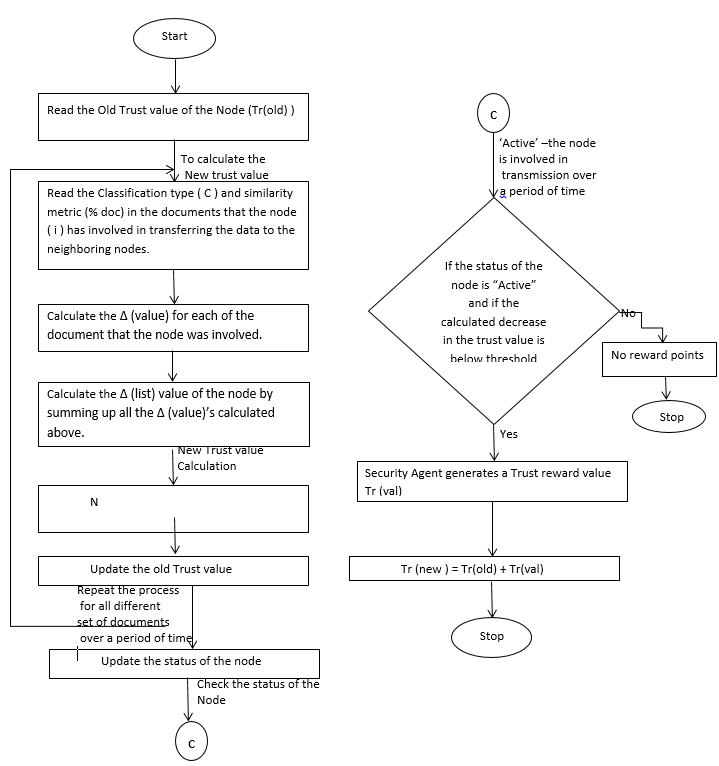
\includegraphics[width=0.90\textwidth]{Figures/Trust_Algorithm.PNG}
        \caption{Trust Evaluation Algorithm}
    \end{center}
\end{figure}
  
\section{Trust Value Testing Results on Various Scenarios}
Table \ref{tab:trust_testing} demonstrates the intermediate steps of calculating
trust. Finally, trust values are updated in Table \ref{tab:trust_evaulation}.
\begin{table}[h!]
    \centering
\begin{tabular}{c | c | c | c | c | c}
    \hline
    Node ID	& DOCUMENT ID	& \( \Delta_{ID} \) 	 & C	& \%doc	& \( \Delta_{value} \) \\
    \hline \hline
1        & 1	&  Doc - 1      & 0.04       & 0.5	& 0.02 \\
1        & 2	&  Doc - 2      & 0.05       & 0.3	& 0.015 \\
1        & 3	&  Doc - 3      & 0.06       & 0.45	& 0.027 \\
\hline
&		&	 	        &            & \textbf{Sum}	& \em{0.062} \\

    \hline
Node ID &	DOCUMENT ID	&  \( \Delta_{ID} \)         & C	& \%doc& \( \Delta_{value} \) \\
\hline \hline
2        &1	  & Doc - 1         & 0.05       & 0.6	& 0.03 \\
2        &2	  & Doc - 2         & 0.08       & 0.8	& 0.064 \\
2        &3	  & Doc - 3         & 0.075      & 0.9	& 0.0675 \\
\hline
&	  &    	            &            & \textbf{Sum}	& 0.\em{1615} \\
    \hline
Node ID &	DOCUMENT ID	&  \( \Delta_{ID} \)         & C	& \%doc	& \(
\Delta_{value} \) \\
\hline \hline
3        &1	  & Doc - 1         & 0.058      & 0.66	& 0.03828 \\
3        &2	  & Doc - 2         & 0.03       & 0.9	& 0.027 \\
3        &3	  & Doc - 3         & 0.095      & 0.2	& 0.019 \\
\hline
& 	  &                 &            & \textbf{Sum}	& \em{0.08428} \\
    \hline
Node ID &	DOCUMENT ID	&  \( \Delta_{ID} \)         & C	& \%doc	 & \(
\Delta_{value} \) \\
\hline \hline
4        &1	  & Doc - 1         & 0.09       & 0.6	& 0.054 \\
4        &2	  & Doc - 2         & 0.045      & 0.44	& 0.0198 \\
4        &3	  & Doc - 3         & 0.095      & 0.77	& 0.07315 \\
\hline
&    &                 &            &	\textbf{Sum}	& \em{0.14695} \\
\end{tabular}

\begin{align*}
    \text{Where}& \\
    C &:= 0 \to 0.1 \\
    D &:= 0 \to 1 \\
    \Delta_{value} &:= C \cdot \%doc
\end{align*}
    \caption{Trust value testing results}
    \label{tab:trust_testing}
\end{table}

\begin{table}[h!]
    \centering
\begin{tabular}{c | c | c | c}
    \hline
    Node ID	& Current Trust Value &	\( \Delta_{List} \) & \( Tr_{new} \)\\
    \hline \hline
1       & 0.45                & 0.062    &    0.388 \\
2       & 0.35                & 0.162    &    0.188 \\
3       & 0.65                & 0.084    &    0.566 \\
4       & 0.5                 & 0.147    &    0.353 \\
\end{tabular}
\caption{Using the results from Table \ref{tab:trust_testing}, trust my be
updated.}
\label{tab:trust_evaulation}
\end{table}
\section{Trust Interface to Planning}
\( X \) is a value calculated using the level obtained through classification and the evaluated trust value of a node.
\begin{equation}
    \label{eq:trust_planning_interface}
    \begin{aligned}
        X &= Tr_{new} + \frac{\ln \frac{l}{L}}{10} \\
    \text{Where}~l &:= \text{Node's level} \\
    L &:= \text{Maximum Level}
    \end{aligned}
\end{equation}
The returned value is between 0 and 1 and is sent as an input to the planning phase.
Table 1 where Maximum level = 10 which belongs to the top most employee or node.
\begin{table}[h!]
    \centering
    \begin{tabular}{c | c | c | c}
        \hline
        Node ID	 & \( Tr{new} \) &	Level &	X \\
\hline \hline
1 &	0.388 &	3	 & 0.26760272 \\
2 &	0.188 &	10	 & 0.188 \\
3 &	0.566 &	2	 & 0.405056209 \\
4 &	0.353 &	2	 & 0.192056209 \\
5 &	0.99  &   1	 & 0.759741491 \\
6 &	0.99  &   10 & 	0.99 \\
7 &	0.01  &   10 & 	0.01 \\
8 &	0.5	  &   1	 & 0.269741491 \\
9 &	0.3	  &   2	 & 0.139056209 \\
\end{tabular}
\caption{Test values for Equation~\ref{eq:trust_planning_interface}}
\label{tab:trust_planning}
\end{table}

From Table~\ref{tab:trust_planning}, it is clear that the returned value for
\( X \) is higher for the more trustworthy nodes. Also, if the trust value is same for
two nodes, then the node, which is superior in level, has a slightly larger
value for \( X \).

\subsection{General References}
The following references provided overall general information to this chapter:
\autocite{JiminLi2010}, \autocite{Varadharajan2004},
\autocite{Varadharajan2005}.

